\uuid{IxMl}
\niveau{PCSI}
\module{Analyse}
\chapitre{Généralités sur les nombres réels}
\sousChapitre{\'Equations et inéquations}
%!TeX root=../../../encours.nouveau.tex
%%% Début exercice %%%

\duree{10}
\difficulte{1}
\auteur{Antoine Crouzet}
\datecreate{01/12/2024}
\titre{Inéquations et valeurs absolues}
\contenu{
\question{Résoudre les inéquations
\[ |2x-5|\leq |x+3| \qeq |x^2-6x+7| < 1 \]}
\reponse{\begin{remarque}
  L'équation $|f(x)|\leq |g(x)|$ est équivalente à l'équation $(f(x))^2\leq (g(x))^2$ car les termes sont positifs.
\end{remarque}
On utilise la remarque précédente :
\begin{align*}
 |2x-5| \leq |x+3| &\Leftrightarrow (2x-5)^2 \leq (x+3)^2 \\
 &\Leftrightarrow (2x-5)^2-(x+3)^2 \leq 0\\
 &\Leftrightarrow ((2x-5)-(x+3))((2x-5)+(x+3)) \leq 0 \\
 &\Leftrightarrow  (x-8)(3x-2) \leq 0
\end{align*}
On dresse un tableau de signes :
\begin{center}
\begin{tikzpicture}
   \tkzTabInit[espcl=1.5,lgt = 3]{$x$ / 0.9 , $x-8$ / 0.7, $3x-2$ / 0.7, $(x-8)(3x-2)$ / 0.7}{$-\infty$, $\dfrac23$, $8$, $+\infty$}
   \tkzTabLine{,-, , -,z,+,}
   \tkzTabLine{,-,z, +,,+,}
   \tkzTabLine{,+,z, -,z,+,}
\end{tikzpicture}
\end{center}
On peut conclure : \[ \boxed{\mathcal{S}= \left [ {\frac{2}{3}},\,8\right ].}\]
Pour la deuxième inéquation, on utilise les propriétés de la valeur absolue :
\[ |x^2-6x+7|<1 \iff -1 < x^2-6x+7 < 1 \iff \left( 0<x^2-6x+8 \qeq x^2-6x+6<0\right). \]
On résout les deux inéquations (trinôme du second degré) :
\begin{align*}
  x^2-6x+8 >0 &\iff x \in \interoo{-\infty{} 2}\cup \interoo{4 +\infty} \\
  x^2-6x+6 < 0 & \iff x \in \interoo{3-\sqrt{3} 3+\sqrt{3}}
\end{align*}
Ainsi,
\[ |x^2-6x+7|<1 \iff x\in \left(\interoo{-\infty{} 2}\cup \interoo{4 +\infty}\right)\cap \interoo{3-\sqrt{3} 3+\sqrt{3}}. \]
\textbf{Bilan} : \[ \boxed{\mathcal{S} = \interoo{3-\sqrt{3} 2}\cup \interoo{4 3+\sqrt{3}}.}\]}
}
